\chapter{RL basado en modelo}

\lecture{11}{2020-06-20}{Model-Based Reinforcement Learning}

\section{Lo básico de RL basado en modelo.}%
\label{sec:lo_básico_de_rl_basado_en_modelo_}

El objetivo es aprender $f(s_t,a_t)=s_{t+1}$ (o $p(s_{t+1}|s_t,a_t)$) ya que conociéndolo se pueden utilizar los
algoritmos vistos en el tema anterior.

Una vista general sencilla (que en la práctica no funciona) es la siguiente:
\begin{enumerate}
    \item Ejecutar la política base $\pi_0(a_t|s_t)$ (por ejemplo aleatoria) para recoger
        $D=\{(s,a,s')_i\}$
    \item Aprender la dinámica $f(s,a)$ de forma que minimice  $\sum_i
        ||f(s_i,a_i)-s_i'||^2$
    \item Planificar con $f(s,a)$ para escoger las acciones.
\end{enumerate}

En el paso 2, en el caso de que se tengan estados discretos la función de pérdida podría pasar
a ser la entropía cruzada, y en el caso de un modelos estocástico cambiaría completamente.

Esto funciona en casos sencillos, como por ejemplo la identificación de sistemas en
robótica. En la que con una política hecha a mano se puede usar para calcular la masa de
los enlaces por ejemplo.

En los casos de dinámica más complejas, para modelarlas se tiene que tener una política que
explore lo suficiente, ya que de lo contrario se pueden quedar estados sin representar. En
estos casos el algoritmo anterior no funciona.

\subsection{El por qué una aproximación sencilla no funciona}%
\label{sub:el_por_qué_una_aproximación_sencilla_no_funciona}

Si se tiene una política $\pi_0(a_t|s_t)$, se generarán muestras del modelo bajo la distribución
de esa política: $p_{\pi_0}(s_t)$. Si la política es pobre, es decir, no hace que se explore
todo lo posible el espacio de estados, a la hora de dejar actuar a la política final es muy
probable que tome acciones pensando que vaya a estados que no son los esperados. Por lo que la
distribución de estados visitados bajo esta nueva política ($p_{\pi_f}(s_t)$) no es la misma y el modelo no ha
sido entrenado bajo esta distribución.

\begin{figure}[H]
	\centering
	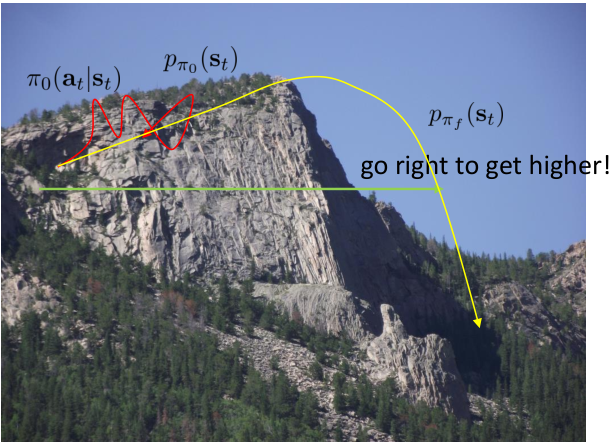
\includegraphics[width=0.5\linewidth]{figures/2020-06-21-205040_611x446_scrot.png}
\end{figure}

Este problema se le conoce \textit{distribution missmatch}, el cual se vuelve más
exacerbado cuanto más expresivo es el modelo que representa el mundo.

El problema se resolvería si $p_{\pi_0}(s_t)=p_{\pi_f}(s_t)$. Para conseguirlo, se
modifica el algoritmo anterior de la siguiente manera (es básicamente DAgger pero para modelos):

\begin{enumerate}
    \item Ejecutar la política base $\pi_0(a_t|s_t)$ (por ejemplo aleatoria) para recoger
        $D=\{(s,a,s')_i\}$
    \item Aprender la dinámica $f(s,a)$ de forma que minimice  $\sum_i
        ||f(s_i,a_i)-s_i'||^2$
    \item Planificar con $f(s,a)$ para escoger las acciones.
    \item Ejecutar esas acciones y añadir las nuevas muestras $\{(s,a,s')_j\}$ a  $D$.
\end{enumerate}

Los pasos 2 a 4 forman un bucle.

Hay una modificación que puede hacerlo funcionar mejor. Consiste en tomar solo una acción y
replanificar para el siguiente estado:

\begin{enumerate}
    \item Ejecutar la política base $\pi_0(a_t|s_t)$ (por ejemplo aleatoria) para recoger
        $D=\{(s,a,s')_i\}$
    \item Aprender la dinámica $f(s,a)$ de forma que minimice  $\sum_i
        ||f(s_i,a_i)-s_i'||^2$
    \item Planificar con $f(s,a)$ para escoger las acciones.
    \item Ejecutar la primera acción y observar el estado resultante $s'$ (MPC).
    \item Añadir las nuevas muestras $\{(s,a,s')_j\}$ a  $D$.
\end{enumerate}

Los pasos 3 a 5 están en un bucle. Existe otro bucle externo entre los pasos 2 y 5, que sirve
para actualizar el modelo del mundo.

MPC significa \textit{Model Predictive Controller}, que quiere decir que se realiza la
planificación en cada paso.

Una planificación que se ejecute en cada paso compensa muy bien las imperfecciones de
las dinámicas del mundo. Además hace que no sea necesario usar horizontes muy distantes.

Normalmente, si se usa una red neuronal para codificar la dinámica del entorno, al comienzo
los modelos basados en modelo aprenderán mejor que los que no están basados en modelo. Pero con
el tiempo se quedan atrapados en un 'máximo local' y son superados por los no basados en
modelo.
Esto se debe principalmente a que al comienzo la red neuronal se sobreentrena con el
\textit{dataset} $D$, que contiene poca experiencia. Lo que hace que el planificador tienda
a escoger falsas altas recompensas.

\begin{figure}[H]
	\centering
	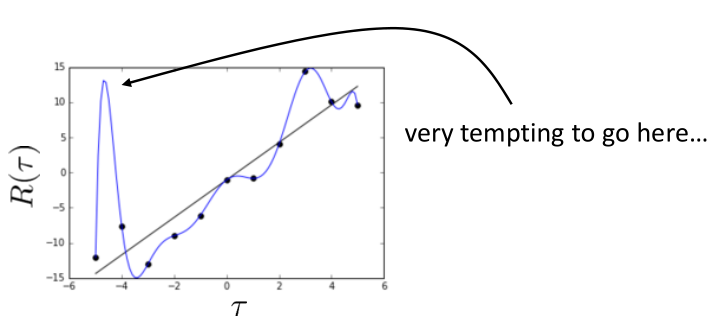
\includegraphics[width=0.5\linewidth]{figures/2020-06-27-171654_723x328_scrot.png}
\end{figure}

Este problema se ve agravado conforme las dimensiones van aumentando. Llega un momento en el que
es la norma sacar valores erróneos en vez de la excepción.

\section{Incertidumbre en RL basado en modelo}%
\label{sec:incertidumbre_en_rl_basado_en_modelo}

Para contrarrestar este problema, en vez de usar un modelo determinista para aproximar el
entorno, se puede usar un modelo probabilístico, en donde se indica un nivel de desconocimiento
en el modelado del mismo.

\begin{figure}[htpb]
	\centering
	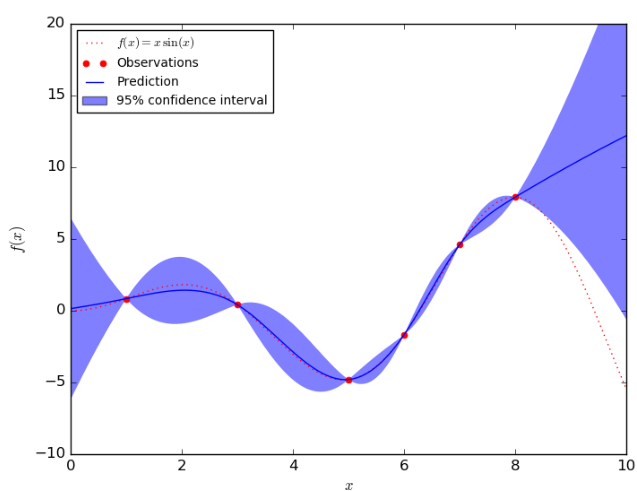
\includegraphics[width=0.5\linewidth]{figures/2020-06-27-172621_637x491_scrot.png}
	\caption{Proceso de gaussianas para modelar la dinámica. No es un método escalable pero
    suficiente para ilustrar.}
\end{figure}

Al tomar la esperanza, se evita que el agente explote las zonas del aproximador que no son
correctas. Además, conforme se vayan recogiendo más muestras, la incertidumbre se irá reduciendo y
las predicciones mejorando.

A la hora de usar este modelo hay que tener lo siguiente en cuenta:
\begin{itemize}
    \item No se tiene un mecanismo para explorar
    \item El valor esperado no es lo mismo que el valor pesimista. Aunque se podría usar para
        tareas críticas. No explora mucho.
    \item El valor esperado no es lo mismo que el valor optimista. Suele explorar más.
    \item La experanza es normalmente un buen comienzo.
\end{itemize}

En el caso de redes neuronales, se puede hacer que sean 'conscientes' de su incertidumbre de
diferentes formas:
\begin{itemize}
    \item Usar la entropía de la salida. Esto no es lo suficientemente bueno porque el modelo
        puede estar seguro (baja entropía) pero tener una salida errónea. La raíz del problema
        está en que hay dos tipos de incertidumbre:
        \begin{itemize}
            \item Incertidumbre estadística o aleatoria: básicamente es incertidumbre sobre
                los datos.
            \item Incertidumbre del modelo o epistemológica: el modelo predice bien los datos, pero
                con ese modelo no se obtienen resultados coherentes.
        \end{itemize}
        Por lo que en el caso de que se sobreeentrene la red, la entropía parecerá ser baja
        pero el modelo no será bueno.
    \item Estimar la incertidumbre del modelo. Cuando se entrenan redes neuronales,
        típicamente se suele hacer con \textit{Maximum Likelihood}, donde se estima
        \[
\operatorname { arg } \operatorname { max } _ { \theta } \operatorname { log } p ( \theta | D ) = \operatorname { arg } \operatorname { max } _ { \theta } \operatorname { log } p ( D | \theta )
        \] 
        ¿Se puede aproximar $p(\theta|D)$? Esto nos da la entropía del modelo. Ya que si se
        tiene que todas las  $\theta$ son igual de probables dado $D$, no se tiene ni idea de
        cuál es el modelo. En caso contrario, si se sabe que una única $\theta$ explica
        $D$, se conoce completamente el modelo. La entropía de $p(\theta|D)$ nos da la
        incertidumbre del modelo. Entonces si se quiere predecir, se hace:
        \[
\int p ( s _ { t + 1 } | s _ { t } , a _ { t } , \theta ) p ( \theta | D ) d \theta
        \] 
        En la práctica es casi imposible hacerlo así.
\end{itemize}

Se va a intentar seguir con la segunda aproximación mediante \textbf{redes neuronales
bayesianas}. 

\begin{figure}[H]
	\centering
	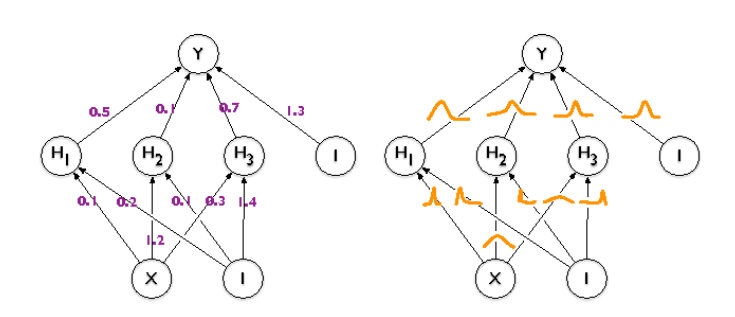
\includegraphics[width=0.8\linewidth]{figures/2020-06-27-180325_735x317_scrot.png}
	\caption{Izqda: red neuronal. Dcha: red neuronal bayesiana}
\end{figure}

En vez de tener un número asociado a cada conexión, se tiene una distribución (sobre
los pesos) asociada a cada conexión. Para hacer este problema realizable en la práctica, se
realiza una aproximación. Una de las simplificaciones más grandes que se puede hacer es
estimar la distribución sobre los parámetros como un producto de marginales independientes:
\begin{align}
p ( \theta | D ) = \prod _ { i } p ( \theta _ { i } | D )\\
p ( \theta _ { i } | D ) = N ( \mu _ { i } , \sigma _ { i } )
\end{align}
Donde $\mu_i$ es la esperanza del parámetro y  $\sigma_i$ la incertidumbre sobre ese parámetro.

Esta simplificación se llama \textit{Mean Field Approximation} y suele usarse en física.

Existen varias formas de entrenar redes neuronales bayesianas, siendo una de las más sencillas
\textbf{bootstrap ensembles}. Formalmente:
\begin{align}
p ( \theta | D ) \approx \frac { 1 } { N } \sum _ { i } \delta ( \theta _ { i } )
\end{align}

Este método consiste en entrenar varios modelos y comprobar
si se ponen de acuerdo.
\begin{align}
\int p ( s _ { t + 1 } | s _ { t } , a _ { t } , \theta ) p ( \theta | D ) d \theta \approx \frac { 1 } { N } \sum _ { i } p ( s _ { t + 1 } | s _ { t } , a _ { t } , \theta _ { i } )
\end{align}

Para entrenar estos modelos, se generan datasets independientes para obtener modelos
'independientes'. Una de las formas de conseguir esto es coger el dataset original $D$ y hacer
un remuestreo con reemplazos.

En resumen:
\begin{itemize}
    \item Este método funciona.
    \item Es una aproximación bastante simplista, ya que normalmente el número de modelos es
        pequeño (<10).
    \item Remuestreo con reemplazo suele ser innecesario. Porque SGD y la inicialización
        aleatoria normalmente hace que los modelos sean lo suficientemente independientes.
\end{itemize}

\subsection{Planificación con incertidumbre}%
\label{sub:planificación_con_incertidumbre}

En el tema anterior, se vio que se necesitaba una estimación de la calidad de una serie de
acciones.
\begin{align}
J ( a _ { 1 } , \ldots , a _ { H } ) = \sum _ { t = 1 } ^ { H } r ( s _ { t } , a _ { t } ) , \text { where } s _ { t + 1 } = f ( s _ { t } , a _ { t } )
\end{align}
Ahora como se tienen $N$ redes neuronales, se saca la media de los modelos:
\begin{align}
J ( a _ { 1 } , \ldots , a _ { H } ) = \frac { 1 } { N } \sum _ { i = 1 } ^ { N } \sum _ { t = 1 } ^ { H } r ( s _ { t , i } , a _ { t } ) , \text { where } s _ { t + 1 , i } = f _ { i } ( s _ { t , i } , a _ { t } )
\end{align}

Lo anterior es para modelos deterministas.

Más generalmente, si se tiene una serie de acciones candidatas $ a_1,\ldots,a_H$:
\begin{enumerate}
    \item Coger una muestra $\theta \sim p(\theta|D)$ 
    \item En cada paso $t$, coger la muestra $s_{t+1}\sim p(s_{t+1}|s_t,a_t,\theta)$.
    \item Calcular $R=\sum_t r(s_t,a_t)$
    \item Repetir los pasos de 1 a 3 y acumular la recompensa media.
\end{enumerate}
Como resultado se tiene la esperanza del valor de la recompensa para la serie de acciones
candidatas en modelos estocásticos y distribuciones sobre los parámetros.

Existen otras opciones de hacer esto: \textit{moment matching}, estimaciones más complejas con
BNN, \ldots

Publicaciones relacionadas:
\begin{itemize}
\item Deisenroth et al. PILCO: A Model-Based and Data-Efficient Approach to Policy Search.
\item Nagabandi et al. Neural Network Dynamics for Model-Based Deep Reinforcement Learning with Model-Free Fine-Tuning.
\item Chua et al. Deep Reinforcement Learning in a Handful of Trials using Probabilistic Dynamics Models.
\item Feinberg et al. Model-Based Value Expansion for Efficient Model-Free Reinforcement Learning.
\item Buckman et al. Sample-Efficient Reinforcement Learning with Stochastic Ensemble Value Expansion.
\end{itemize}

\section{RL basado en modelo con observaciones complejas}%
\label{sec:rl_basado_en_modelo_con_observaciones_complejas}

En el caso de que se quieran controlar robots con cámaras, o jugar a Atari, las observaciones se
vuelven muy complejas. Si se quiere aprender $f(s_t,a_t)=s_{t+1}$, siendo  $s$ imágenes por
ejemplo, la tarea se complica por la alta dimensionalidad, la redundancia y la observabilidad
parcial (en Atari por ejemplo con una imagen no se puede saber la velocidad de la bola).

\subsection{State space (latent space) models}%
\label{sub:state_space_latent_space_models}

Se podría aprender de forma separada $p(o_t|s_t)$ y  $p(s_{t+1}|s_t,a_t)$. Esto puede ser bueno
porque el primer término tiene una alta dimensionalidad pero no es dinámico, mientras que el
segundo puede ser más complejo por la dinámica pero tiene una dimensionalidad
mucho más reducida. Para verlo, se puede pensar que en el estado queda codificada la
posición de la pala del juego de Atari Breakout mientras que la observación son los píxeles en
sí.

Aunque puede ser que esta no sea la aproximación que se tome siempre (ver final del tema).

A la hora de implementar este método, también se necesita aprender la probabilidad de la
recompensa dado el estado actual y la acción: $p(r_t|s_t,a_t)$.

\begin{figure}[H]
	\centering
	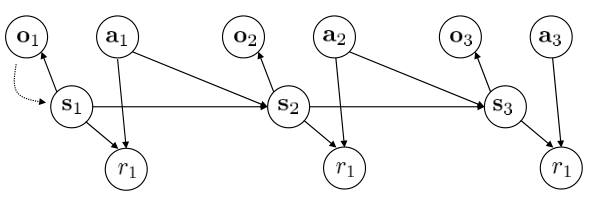
\includegraphics[width=0.5\linewidth]{figures/2020-06-27-194435_590x198_scrot.png}
\end{figure}

\subsubsection{¿Cómo se entrena?}%
\label{ssub:_cómo_se_entrena_}

Anteriormente, cuando se tenía un modelo totalmente observable, se entrenaba bajo ML:
\begin{align}
\max _{\phi} \frac{1}{N} \sum_{i=1}^{N} \sum_{t=1}^{T} \log p_{\phi}\left(\mathbf{s}_{t+1, i} \mid \mathbf{s}_{t, i}, \mathbf{a}_{t, i}\right)
\end{align}
Ahora se tiene que introducir algo más complejo, \textit{expected log-likelihood}:
\begin{align}
    \max _{\phi} \frac{1}{N} \sum_{i=1}^{N} \sum_{t=1}^{T} E_{(s_t,s_{t+1})\sim
    p(s_t,s_{t+1}|o_{1:T},a_{1:T})}\left[\log p_{\phi}\left(\mathbf{s}_{t+1, i} \mid \mathbf{s}_{t, i}, \mathbf{a}_{t, i}\right)+\log p_{\phi}\left(\mathbf{o}_{t, i} \mid \mathbf{s}_{t, i}\right)\right]
\end{align}
La esperanza con respecto a $(s_t,s_{t+1})\sim p(s_t,s_{t+1}|o_{1:T},a_{1:T})$ hace que el
entrenamiento sea muy complicado.

Esto se suele hacer aprendiendo un posterior aproximado $q_\phi(s_t|o_{1:t},a_{1:t})$ (a veces
llamado \textit{encoder}). Existen distintas opciones para aproximar el posterior:
\begin{itemize}
    \item $q(s_t,s_{t+1}|o_{1:T},a_{1:T})$:  \textit{full smoothing posterior}. Es más
        preciso pero más complicado de implementar.
    \item $q_\phi(s_t|o_t)$: encoder de un paso. Es el más simple, pero menos preciso.
\end{itemize}

Estos \textit{encoders} también se tienen que entrenar, ello se discutirá en el siguiente tema.

A continuación se muestra como entrenar el encoder de un paso. Por lo que la esperanza se obtiene
a partir de
$\mathbf{s}_{t} \sim q_{\psi}\left(\mathbf{s}_{t} \mid \mathbf{o}_{t}\right), \mathbf{s}_{t+1} \sim q_{\psi}\left(\mathbf{s}_{t+1} \mid \mathbf{o}_{t+1}\right)$
Se considera que en este caso $q(s_t|o_t)$ es determinista.
\begin{align}
q_{\psi}\left(\mathbf{s}_{t} \mid
\mathbf{o}_{t}\right)=\delta\left(\mathbf{s}_{t}=g_{\psi}\left(\mathbf{o}_{t}\right)\right)
\implies s_t = g_\phi(o_t)
\end{align}

Por lo que queda:
\begin{align}
\max _{\phi, \psi} \frac{1}{N} \sum_{i=1}^{N} \sum_{t=1}^{T} \log p_{\phi}\left(g_{\psi}\left(\mathbf{o}_{t+1, i}\right) \mid g_{\psi}\left(\mathbf{o}_{t, i}\right), \mathbf{a}_{t, i}\right)+\log p_{\phi}\left(\mathbf{o}_{t, i} \mid g_{\psi}\left(\mathbf{o}_{t, i}\right)\right)
\end{align}

Todo es diferenciable y se puede entrenar con retropropagación.

\begin{figure}[htpb]
	\centering
	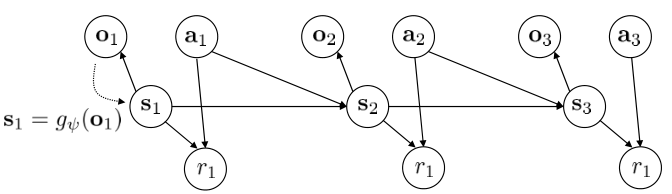
\includegraphics[width=0.5\linewidth]{figures/2020-06-27-201418_672x194_scrot.png}
\end{figure}

\begin{align}
\operatorname { max } _ { \phi , \psi } \frac { 1 } { N } \sum _ { i = 1 } ^ { N } \sum _ { t = 1 } ^ { T } \operatorname { log } p _ { \phi } ( g _ { \psi } ( o _ { t + 1 , i } ) | g _ { \psi } ( o _ { t , i } ) , a _ { t , i } ) +
\end{align}
El primer término se corresponde con el espacio latente de la dinámica, el segundo con la
reconstrucción de la imagen y el tercero con el modelo de la recompensa.

\begin{algorithm}
    \caption{RL basado en modelo con espacio latente de modelos}
    Ejecutar la política base $\pi_0(a_t|o_t)$ (por ejemplo aleatorio) para recoger
    $D=\{(o,a,o')_i\}$\\
    \While{se siga entrenando}{
        Aprender $p_\phi(s_{t+1}|s_t,a_t),p_\phi(r_t|s_t),p(o_t|s_t),g_\psi(o_t)$\\
        \While{no se haya repetido $N$ veces}{
            Planificar según el modelo para escoger las acciones\\
            Ejecutar la primera acción de la planificación, observar la $o'$ resultante (MPC)\\
            Añadir $(o,a,o')$ al dataset $D$.
        }
    }
\end{algorithm}

\subsection{Aprender directamente en el espacio de observaciones}%
\label{sub:aprender_directamente_en_el_espacio_de_observaciones}

En este caso, se aprende directamente $p(o_{t+1}|o_t,a_t)$. Esto puede funcionar
razonablemente bien.

Por ejemplo se puede entrenar una red recurrente gigante para que haga predicciones de
video.
